% 0684(본책 95쪽) — 포물선 y=ax^2 (a>0) 과 직선 y=x+6 의 교점 A·B, B 에서 x축에 내린 수선의 발 H, A 에서 선분 BH 에 내린 수선의 발 C. 라벨은 원문의 O·A·B·C·H·α·β·x·y 와 두 식뿐. 스캔 그림이라 TikZ 로 다시 그림.
% 포물선의 폭은 답(α, β)이 읽히지 않게 원문과 다른 임의 비율(a=1)로 둠.
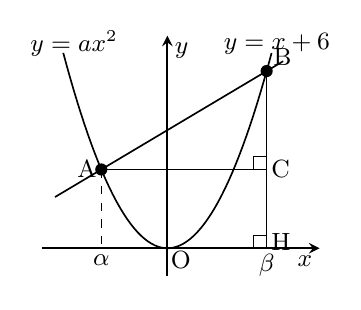
\begin{tikzpicture}[x=0.42cm, y=0.25cm, line width=0.5pt]
  \draw[->, >=stealth, line width=0.7pt] (-3.8,0) -- (4.6,0) node[below left=-1pt, font=\small] {$x$};
  \draw[->, >=stealth, line width=0.7pt] (0,-1.4) -- (0,10.8) node[below right=-1pt, font=\small] {$y$};
  \node[below right, font=\small, inner sep=1pt] at (0,0) {$\mathrm{O}$};
  \draw[line width=0.6pt, domain=-3.15:3.15, samples=60] plot (\x, {\x*\x});
  \draw[line width=0.6pt] (-3.4,2.6) -- (3.5,9.5);
  \draw[line width=0.6pt] (3,9) -- (3,0);
  \draw[line width=0.6pt] (-2,4) -- (3,4);
  \draw[dashed, line width=0.4pt] (-2,4) -- (-2,0);
  \draw (3,4) ++(-0.4,0) -- ++(0,0.65) -- ++(0.4,0);
  \draw (3,0) ++(-0.4,0) -- ++(0,0.65) -- ++(0.4,0);
  \fill (-2,4) circle (2.2pt);
  \fill (3,9) circle (2.2pt);
  \node[left, font=\small, inner sep=1.5pt] at (-2,4) {$\mathrm{A}$};
  \node[above right, font=\small, inner sep=1pt] at (3.1,9.1) {$\mathrm{B}$};
  \node[right, font=\small, inner sep=1.5pt] at (3,4) {$\mathrm{C}$};
  \node[right, font=\small, inner sep=1.5pt] at (3,0.3) {$\mathrm{H}$};
  \node[below, font=\small, inner sep=2pt] at (-2,0) {$\alpha$};
  \node[below, font=\small, inner sep=2pt] at (3,0) {$\beta$};
  \node[left, font=\small, inner sep=1pt] at (-1.4,10.4) {$y=ax^2$};
  \node[right, font=\small, inner sep=1pt] at (1.6,10.4) {$y=x+6$};
\end{tikzpicture}
